\documentclass{article}
\usepackage[utf8]{inputenc}

\title{CSE 344 SYSTEM PROGRAMMING}
\author{HOMEWORK 05 - REPORT }
\date{GÖKHAN HAS - 161044067}

\usepackage{natbib}
\usepackage{graphicx}

\begin{document}

\maketitle

\section{Problem Solutions}
\paragraph{}
In the homework, I got the number of florists by reading the file at first. Then I created my arrays. I kept it all as a global pointer. Actually, I had struct at first. But especially when the ctrlc signal came in, sometimes it wasn't completely free in the memory leak test. In order to prevent this, I went to such a solution.

\paragraph{}
Then I read the file one by one and initialized everything. I created as many threads as the number of florists. I also created the condition variable and mutex as much as the number of florists and initialized them.

\paragraph{}
The wish list is created one by one. The distance is calculated before it is created. Here Chebyshev distance is used. Then, the smallest distance is taken by comparing all the distances. This means that it is the closest florist that sells the same flower. This is also required from us in homework.

\paragraph{}
A problem arises here. Sometimes, no seller can sell the flower that the customer wants. I also checked this. If florists do not sell the flower they want, for example, it cannot be calculated. Since this distance is not calculated, the index does not return in the florist array. So the thread cannot be awakened. Because no florist will be able to serve that customer. Because they don't sell.

\paragraph{}
Then the calculated florist thread is awakened. This is of course done using the cwait function. One two-dimensional integer array was used before being awakened. This array serves as client queue. All of its elements are initially filled with -1. Then the client in the sequence added to the queue is changed to 1. This variable has been defined globally. A separate mutex has been defined since both threads and the main function can access and change. Mutex lock is used when the client queue variable is interfered with. Thus, anyone can interfere with this variable without creating any trouble.

\paragraph{}
All resources received must be returned. This process is done at the end of the mains by destroying mutex and condition variables and using the free function. In case of any signal (ctrlc) these operations should be done and done again.

\paragraph{}
The thread function takes an index as a parameter and returns a struct that contains the information of that thread, that is, the products that the florist sells. In other words, the total sales figure and the total time are returned from the thread. Some control has been done in this function. When the CTRLC signal is received, the thread quits immediately, leaving the requests they are making. If everything goes normally, it makes his requests and leaves.

\paragraph{}
A global flag is marked in the signal function, the signal handler. This flag is checked continuously in threads. As the CTRLC signal (SIGINT) arrives at any time, the threads terminate because the value of the flags will change. After the threads are terminated, the program returns everything it uses. So there is no memory leak process. The screenshots of the tests related to this are available below. There is no memory leak when there is both normal and signal termination.

\section{Used Functions}
\begin{itemize}
    \item void printUsage (): Prints the program's proper usage if it is misused.
    \item void errorExit (char * error): The program should give an error message and terminate cleanly.
    \item int getFloristCount (FILE * fptr, int * countMaxFLower): The number of flowers is taken from the file.
    \item void initializeArrays (int count, int countClient, int maxFlowerCount): Arrays are initialized. Each of them takes place in malloc.
    \item void freeArrays (int count, int clientCount, int maxFlowerCount): When the program is finished or terminated with ctrl + c, the received places are returned by this function.
    \item int getClientCount (FILE * fptr): The number of customers is returned.
    \item void readFile (FILE * fptr, int floristCount, int clientCount): The file is read and the import is done to the arrays. It should not be forgotten that the order of requests will be created one by one again.
    \item int getChCount (char * line, char ch): If there is a few of the value entered as a parameter in the string, it is returned.
    \item void * florist (void * index): The function where threads will run.
    \item void endSignals (int floristCount): If the request list is short or sometimes the request part is made in the main, threads may not work by not entering an interrupt. To prevent this, the condition variable in the threads must be awakened again ...
    \item double getChebyShevDistance (double x1, double y1, double x2, double y2): Chebyshev distance is calculated, the process is made with the shortest distance in the machine.
    \item int isQueueHasElement (int index, int clientCount): It is checked if there is any element in the request list, if it is not, thread should be put into action.
    \item void printInfo (int count, FloristEndInfo * infoArr): The last informative messages are printed.
    \item void signal\_catcher (int sigNo): Signal capture function, SIGINT signal is captured.
\end{itemize}




\begin{figure}[h!]
\centering
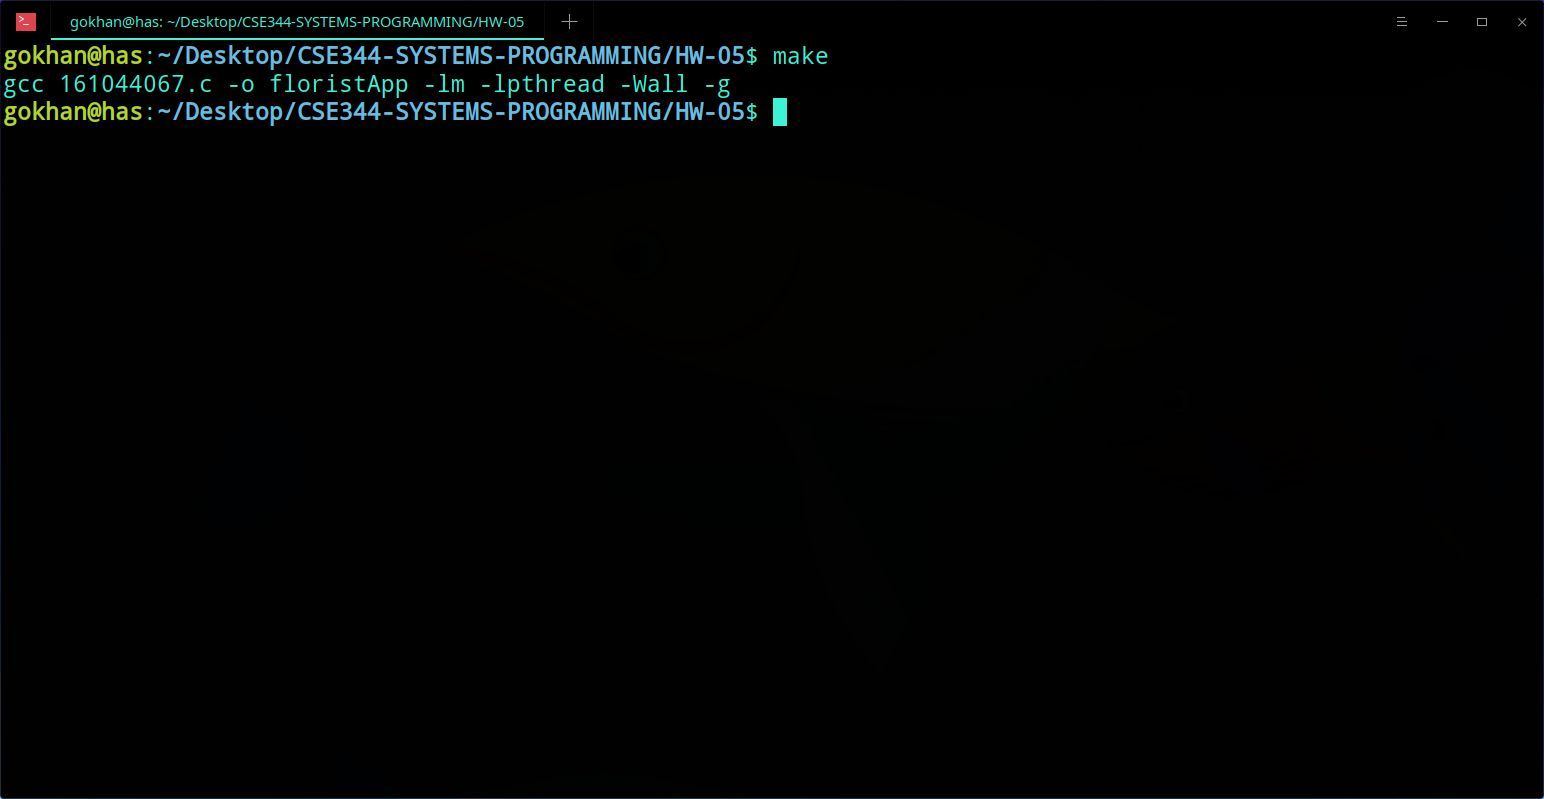
\includegraphics[scale=0.3]{compile.png}
\caption{Compile}
\label{fig:compile}
\end{figure}

\begin{figure}[h!]
\centering
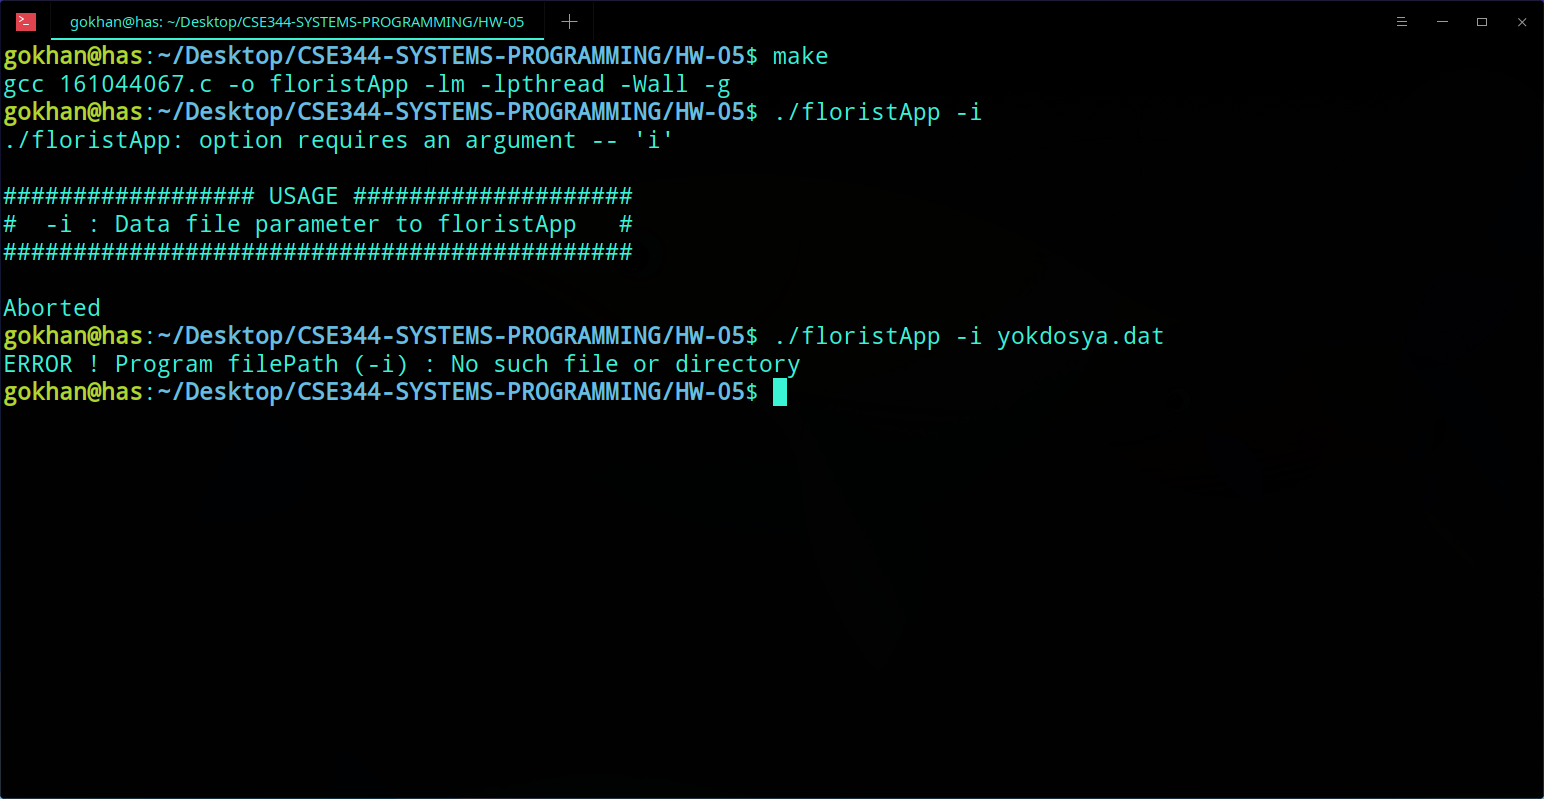
\includegraphics[scale=0.33]{wronginput.png}
\caption{Wrong Input Example}
\label{fig:compile}
\end{figure}

\begin{figure}[h!]
\centering
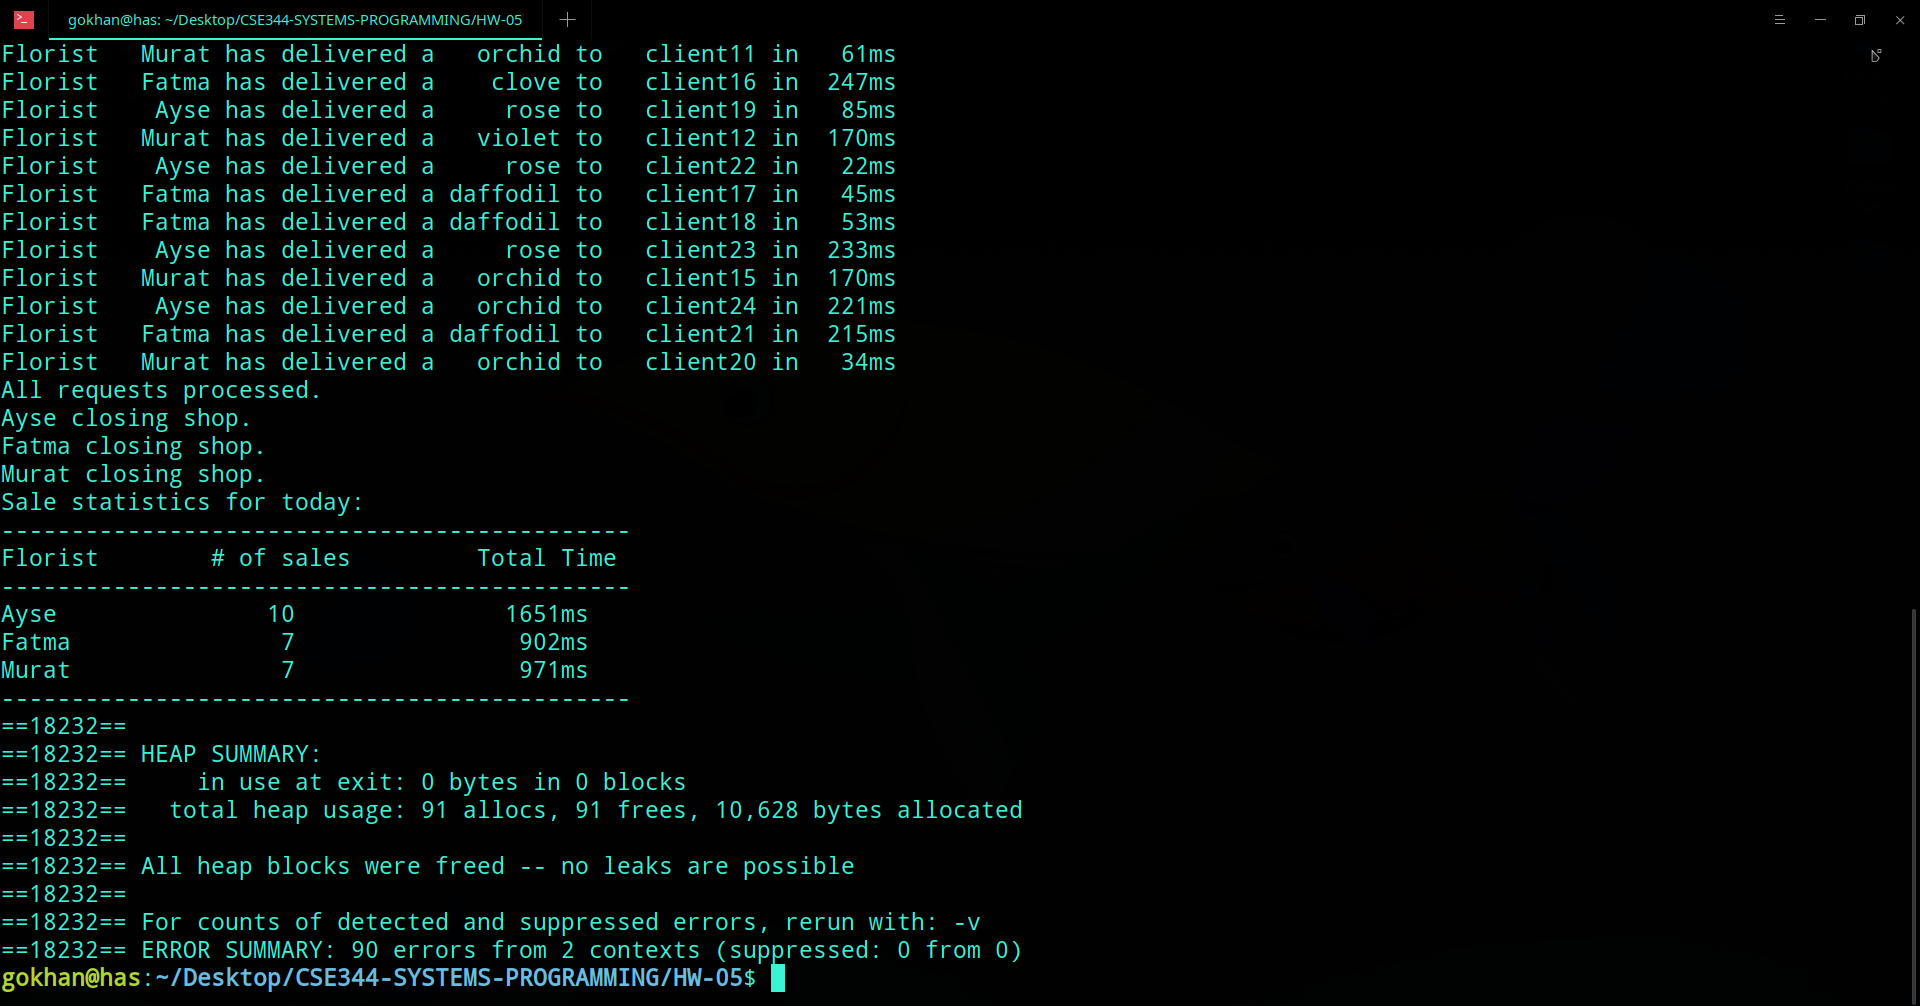
\includegraphics[scale=0.27]{normalleaktest.png}
\caption{Normal Leak Test}
\label{fig:compile}
\end{figure}

\begin{figure}[h!]
\centering
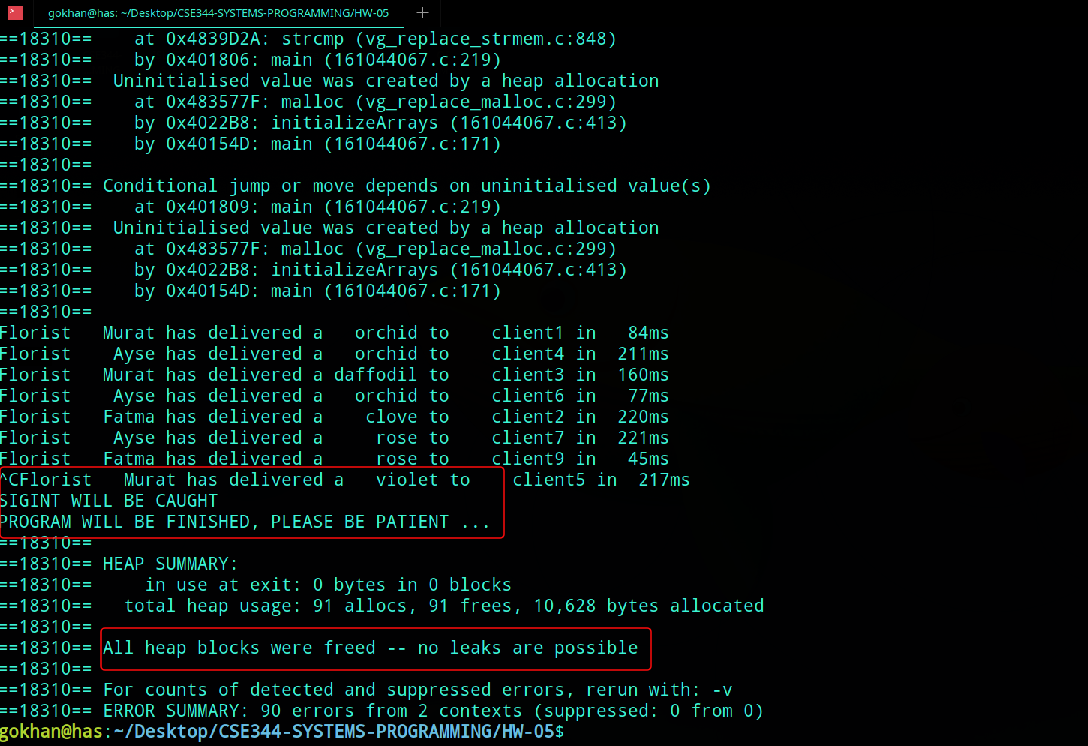
\includegraphics[scale=0.4]{signalleaktest.png}
\caption{Signal Leak Test}
\label{fig:compile}
\end{figure}

\begin{figure}[h!]
\centering
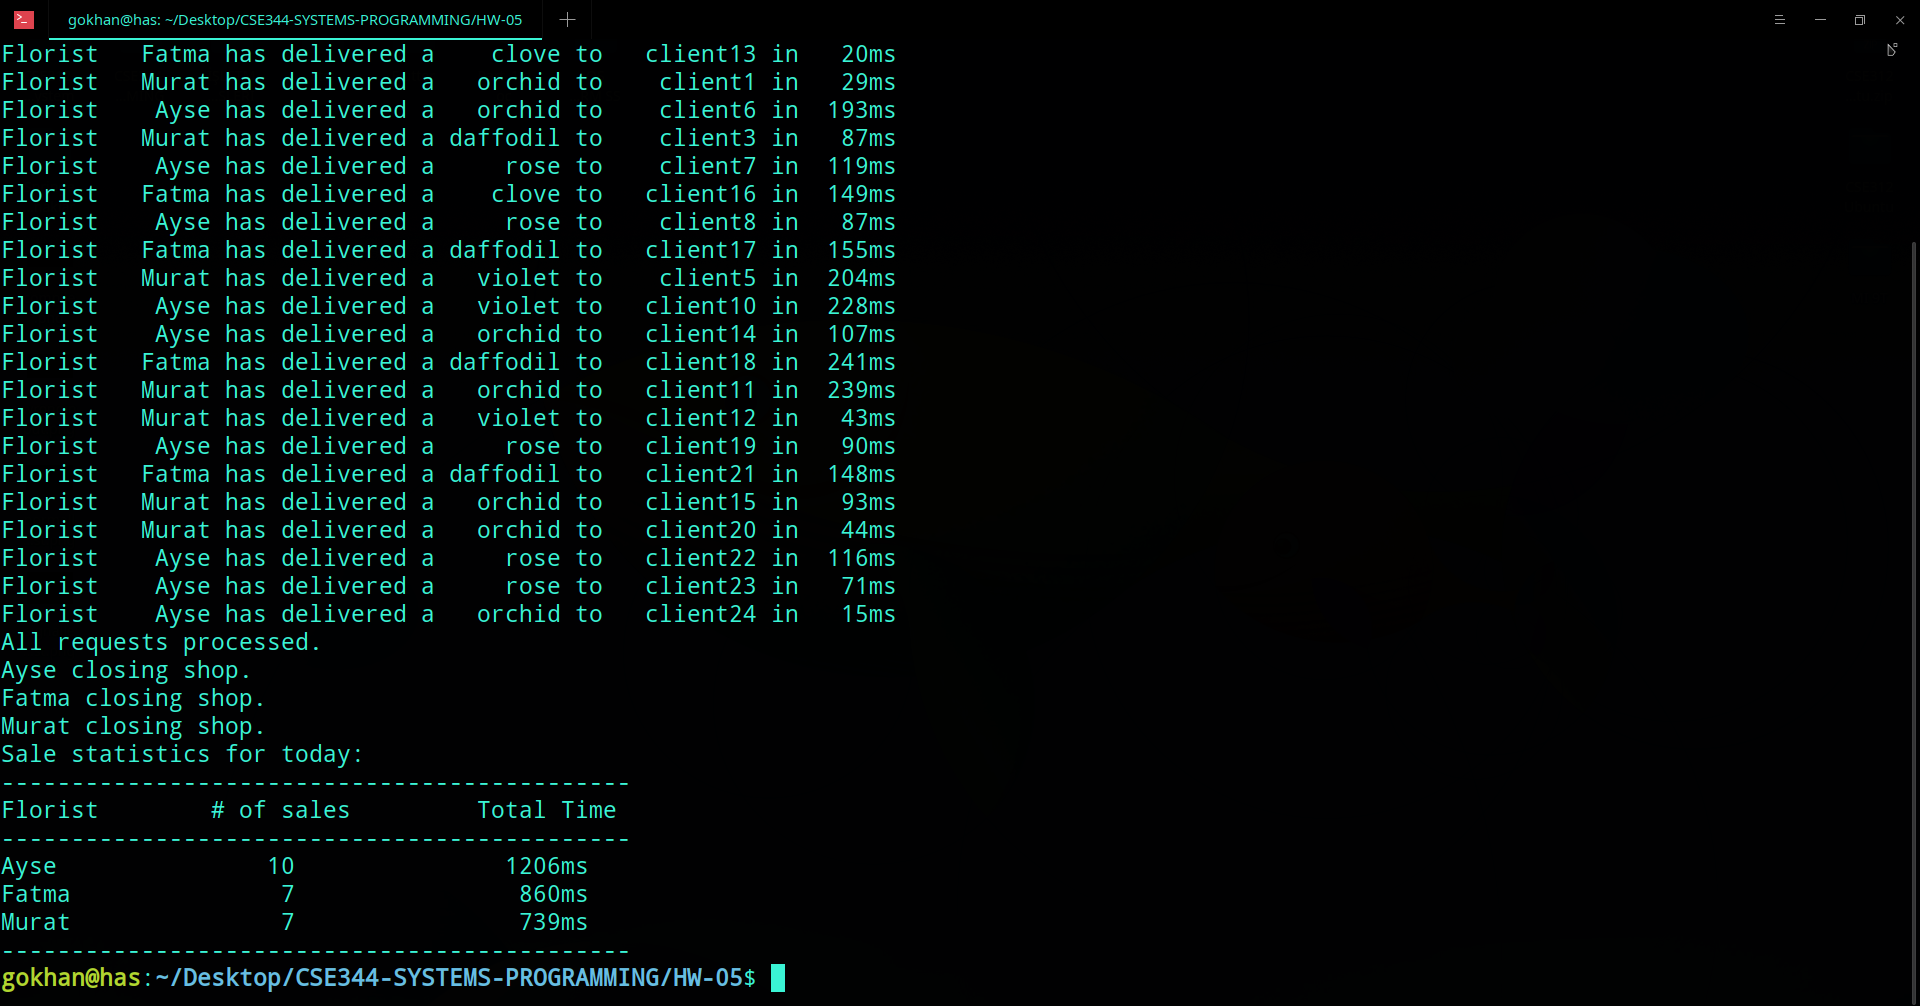
\includegraphics[scale=0.25]{normal.png}
\caption{Normal Test}
\label{fig:compile}
\end{figure}

\begin{figure}[h!]
\centering
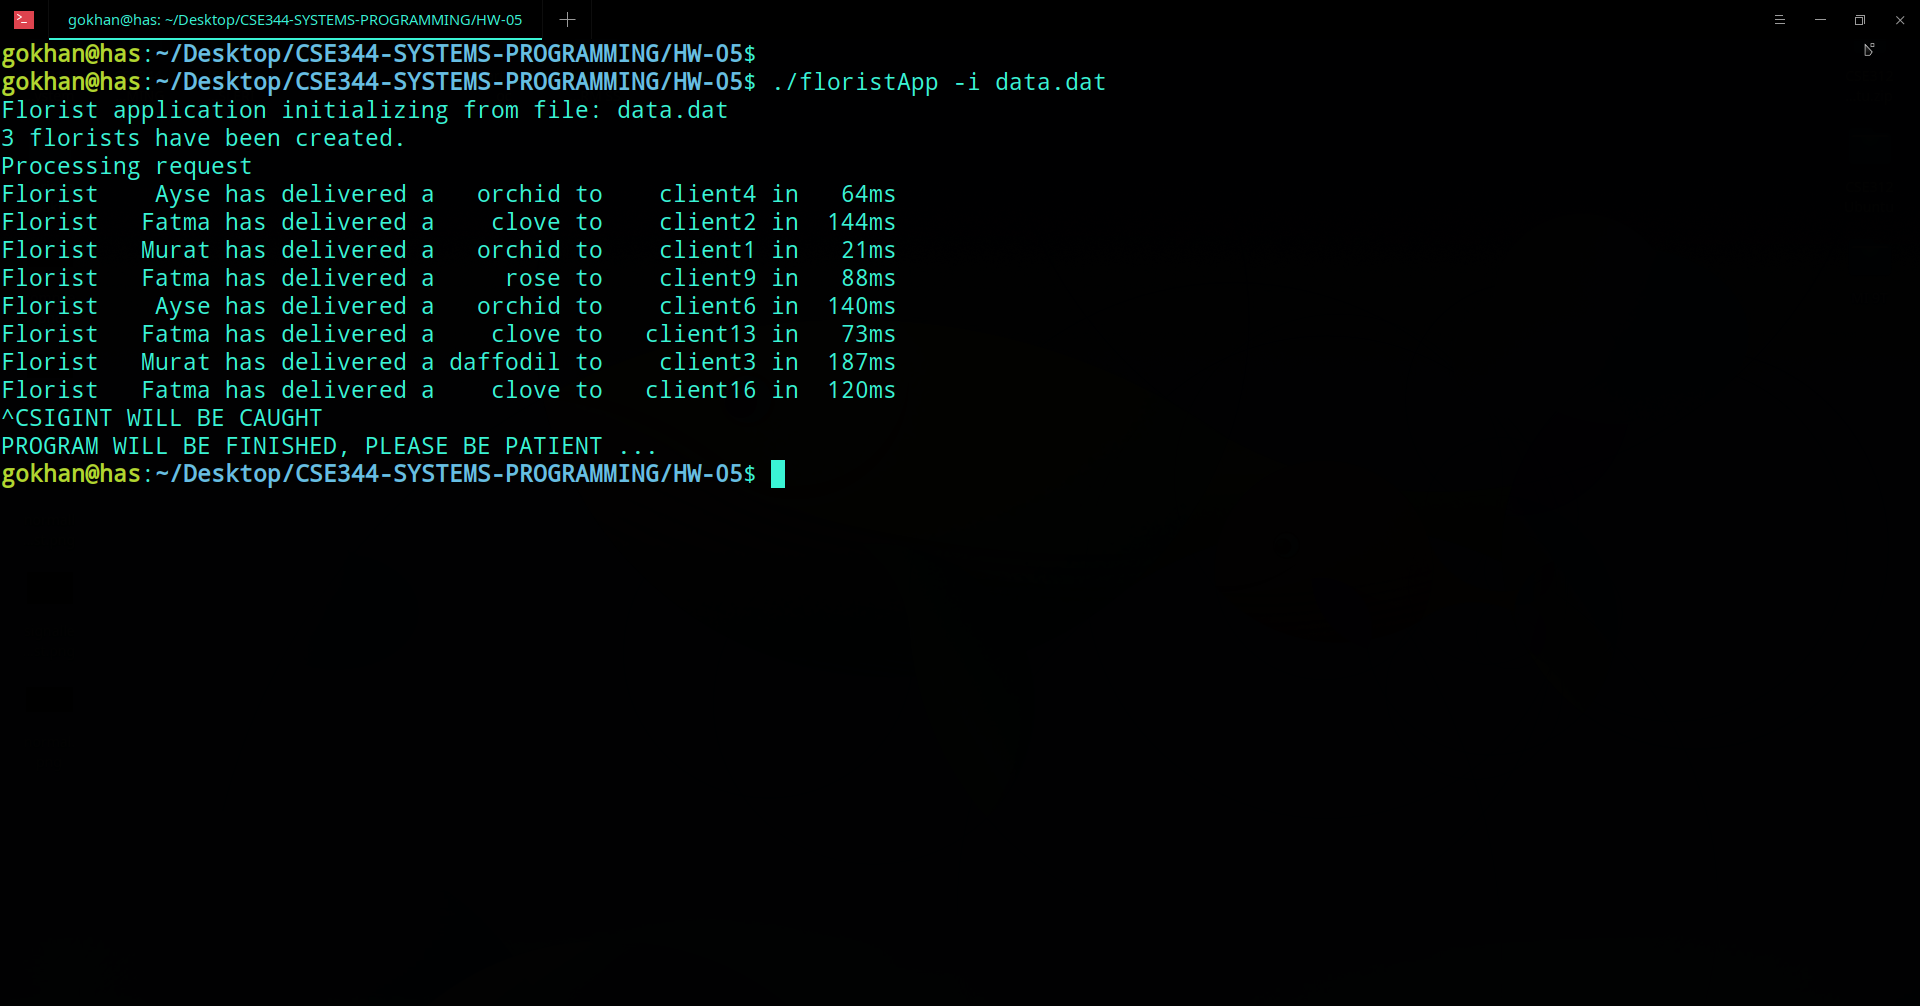
\includegraphics[scale=0.25]{normalsignal.png}
\caption{Normal Signal Test}
\label{fig:compile}
\end{figure}

\bibliographystyle{plain}
\end{document}
